\section{GAME EQUIPMENT}

\subsection{THE GAME MAP}

The 22"x32" mapsheet portrays the area in which the battle was fought. It includes all the significant terrain in the battle. It also displays the Terrain Key and the Turn Record Track.

A hexagonal grid is superimposed over the terrain features printed on the mapsheet in order to regularize movement and positioning of the playing pieces.

To make the map lie flat, back-fold it against the creases. Small pieces of masking tape may be used at the corners of the map to hold it taut.

\subsection{GAME CHARTS AND TABLES}

Various visual aids are provided for the Players in order to simplify and illustrate certain game functions. These are the Terrain Effects Chart, the Combat Results Table, the Reinforcement Chart and the Turn Record Track.

\subsection{THE PLAYING PIECES}

The cardboard pieces represent the actual military units that took part in the original battle. The numbers and symbols on the pieces represent the strength, movement capability and type of unit represented by that piece. These playing pieces will hereafter be referred to as "units".

\subsection{HOW TO READ THE UNITS}

GERMAN UNIT

\begin{center}
  
\includegraphics[scale=0.7]{german_unit_explained.png}
\end{center}

SOVIET UNIT (TRIED)

\begin{center}
  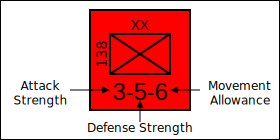
\includegraphics[scale=0.7]{soviet_unit_explained.png}
\end{center}

SOVIET UNIT (UNTRIED)

SOVIET LEADER

\textbf{Unit Designations}
These are the actual identity numbers of the units; divisions have but one number, while regiments have both their regimental identity and the number of the division of which they are a part (the number to the right of the slash is the division I.D.). For example, 20/12 indicates the 20th Panzer Regiment, which was part of the 12th Panzer Division.

\textbf{Unit Types}

Soviet Infantry

Infantry (Motorized)

Armor (Panzer)

Mechanized (Panzer Grenadier)

Air Interdiction Marker

Disruption Marker

Cavalry

German Infantry

\textbf{Unit Sizes}
III=Regiment; XX=Division.

\textbf{Attack Strength} is the relative strength of a unit when attacking, expressed in terms of Strength Points.

\textbf{Defense Strength} is the relative strength of a unit when defending.

\textbf{Combat Strength} is the relative strength of a unit when attacking or defending.

\textbf{Untried Strength}, represented by a question mark; the true strength of the unit is revealed to both Players only after that unit has participated in combat.

\textbf{Leadership Value} is the rating of a particular leader, expressed in Leadership Points.

\subsection{PARTS INVENTORY}

The complete game of \textbf{Panzergruppe Guderian} should include the following parts:
22"x32" Game Map
Rules Folder
Sheet of Die-Cut Counters (200 pieces, printed back and front)
Game Box (not included in the subscription edition)
Plastic Die (not included in the subscription edition)

If any parts are missing or damaged, please write:
Customer Service
Simulations Publications, Inc.
44 East 23rd Street
New York, N.Y. 10010

Questions regarding the rules of the game will be answered if accompanied by a stamped, self-addressed envelope and if phrased to be answered by a simple one word answer. Send rules questions to the above address and mark the envelope "Rules Questions: Panzergruppe Guderian".